\documentclass[a4paper,10pt,oneside]{jsbook}
%
\usepackage{amsmath,amssymb,bm}
\usepackage{bm}
\usepackage[dvipdfmx]{graphicx}
\usepackage{ascmac}
\usepackage{makeidx}
\usepackage{txfonts}
\usepackage{indentfirst}
\usepackage{booktabs}
\usepackage{tabularx}
\usepackage{comment}
\AtBeginDvi{\special {pdf:tounicode EUC-UCS2}}
\usepackage[dvipdfmx, setpagesize=false, bookmarks=true, bookmarksnumbered=true]{hyperref}
\usepackage{nameref}
\usepackage{url}
%
\makeindex
%
\newcommand{\diff}{\mathrm{d}}            %微分記号
\newcommand{\divergence}{\mathrm{div}\,}  %ダイバージェンス
\newcommand{\grad}{\mathrm{grad}\,}       %グラディエント
\newcommand{\rot}{\mathrm{rot}\,}         %ローテーション
%
\setlength{\textwidth}{\fullwidth}
\setlength{\textheight}{44\baselineskip}
\addtolength{\textheight}{\topskip}
\setlength{\voffset}{-0.6in}
%

\begin{document}

%%%%%%%%%%%%%%%%%%%%%%%%%%%%%%%%%%%%%%%%%%%%%%%%%%%%%
% 表紙
\begin{titlepage}
\noindent
独立行政法人 理化学研究所 御中
\begin{center}
	\vspace{8cm}
	{\Huge \textbf{協調ワークスペースドライバと}} \\
	\vspace{1cm}
	{\Huge \textbf{協調動作フレームワークのプロトタイプ}} \\
	\vspace{1cm}
	{\Huge \textbf{操作説明書}} \\
	\vspace{10cm}
	{\Large \textbf{2015年3月26日}} \\
	\vspace{0.5cm}
	{\Large \textbf{株式会社イマジカ デジタルスケープ}}
\end{center}
\end{titlepage}

%%%%%%%%%%%%%%%%%%%%%%%%%%%%%%%%%%%%%%%%%%%%%%%%%%%%%
% 目次
\tableofcontents

%%%%%%%%%%%%%%%%%%%%%%%%%%%%%%%%%%%%%%%%%%%%%%%%%%%%%
% 本文
%%%%%%%%%%%%%%%%%%%%%%%%%%%%%%%%%%%%%%%%%%%%%%%%%%%%%
\chapter{はじめに}
本書では協調ワークスペースドライバと協調動作フレームワークのプロトタイプの操作方法について解説します.

\section{動作環境とインストール}
以下の環境で動作します.

[TODO]

\begin{tabbing}
0123\=01234567890123\=0123456789\kill
\> OS \> : Linux, Windows(Vista,7,8), MacOSX \\
\> Webブラウザ \> : Mozilla Firefox 15.x, Google Chrome 21.x, Apple Safari 6.x, Windows Internet Explorer 10.x 
\end{tabbing}

\section{インストール}

\subsection{Node.jsのインストール}
ポータルGUIの動作にはNode.jsのインストールが必要です.\\
Node.jsの公式サイト(\verb+http://nodejs.org/+)からNode.js本体をダウンロードし,インストールします.

\subsection{プログラムの展開}

TODO:

\subsection{Node.jsサブモジュールのインストール}
アプリケーションを展開したディレクトリに,
ポータルGUIで利用しているNode.jsの必要なサードパーティモジュールのインストールを行います.

TODO:

\begin{verbatim}
   $cd bin
   $sh install.sh 
   (Windows版は install.bat)
\end{verbatim}

\newpage

\section{起動}
起動スクリプトを実行するとポータルGUIサーバーが起動します.
\begin{verbatim}
   $sh run.sh
   (Windows版は run.bat)
\end{verbatim}

\section{コントローラへアクセス}
ポータルGUIは,Webブラウザのアドレス欄に「http://localhost:8080」と入力することでアクセス出来ます.\\

TODO:

\chapter{ホーム画面}
\section{概要}
ホーム画面では,以下の操作を行う事が出来ます.

\begin{itemize}
\item コントローラ画面へ
\item ディスプレイ画面へ
\end{itemize}

\section{操作}

TODO:

\begin{figure}[htbp]
	\begin{center}
		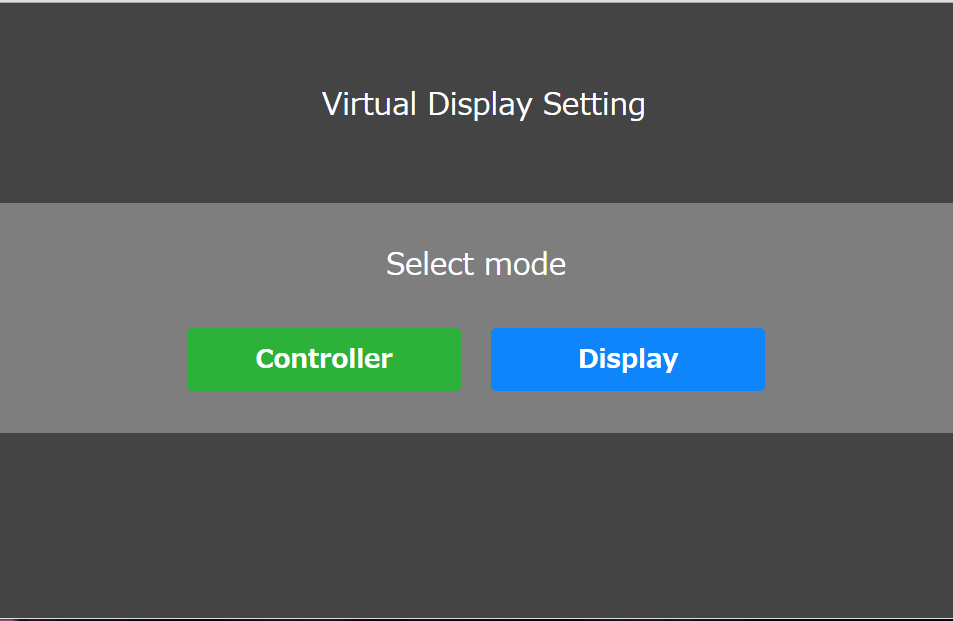
\includegraphics[width=11.5cm]{image/home.png}
	\end{center}
	\caption{ホーム画面}
	\label{fig:home}
\end{figure}


\end{document}

